% !TeX root = ../main.tex

% questions for Asher
% 1. references for the idea that variabilty is inherntly greater in biologicL rather than chemical or physical tests.
%todo TOC/SOC, our/my, we/I


%\section{Preliminary incubation}

\section{effect of management history on \gls{som} pools in non-amended soils}

	\subsection{Cultivated compared with non-cultivated}
	%todo how to cite this 'Seven-years of productivity and potential fertility in organically managed...' (ask Asher)
	Despite my expectations, both cultivated LTTs and especially ORG had resulted in higher baseline values for most parameters, compared with the non-cultivated LTT. Although agricultural intensification and long term fertilization has been repeatedly shown to diminish overall soil health and cause a reduction in \gls{som}, compared with non-cultivated soils \citep{laurance2014, mganga2016, tilman2011}, there is some evidence pointing out that this is not necessarily the case for certain agricultural management scenarios, particularly in arid and semi-arid environments.  For example, \citet{trivedi2016}, in a meta analysis, found that in arid climates, cultivated soils had on average significantly higher values of SOC compared with unmanaged soils. Similarly, repeated analysis of a large data base from soils in the US great plains area, revealed that SOC loss due to cultivation was lowest in low rainfall areas ($ \sim $300 mm \acrshort{map})\citep{miller2004, burke1989}. \citet{paz-kagan2014} conducted a research that included soils from the Migda research farm (\~{}30 km from the Gilat Research Center, with similar climatic conditions and soil properties), and found no significant improvement in Soil Quality Index(SQI) (including soil parameters such as \gls{soc}, hydraulic conductivity and surface hardness) when transitioning between agricultural land use and a natural ecosystem management. \citet{garcia-orenes2010} found no significant decrease in soil health parameters (TOC, WEOC, MBC, basal respiration) compared with an adjacent abandoned field (some natural vegetation cover) in soils from SW Portugal, treated for one year by  a number of different agricultural practices, including tillage and herbicide use. Although these different treatments were each tested separately (e.g compare tilled soil to non-cultivated soil),as opposed to combined long-term treatments in the current work (e.g. compare conventional management to unmanaged soil ), and lasted for only one year, nonetheless, the outcome of this work, clearly support the notion that certain agricultural practices may not have a detrimental effect on overall soil health when compared with non-cultivated soils in a semi-arid climate context. Indeed some practices - such as the work of \citeauthor{garcia-orenes2010}, the return of substantial amount of oat straw - can actually cause a significant improvement in soil health parameters, not just compared with a non-cultivated soil, but also compared with a natural cover soil ( Mediterranean woodland ).\\
	My results provide additional evidence supporting a similar line of evidence. Five years of intense compost application ( $ 6 m^3*year^{-1} $ ) combined with an otherwise conventional management system (Org), increased TOC by almost 60\% over an adjacent uncultivated soil (UNC). Org had also resulted in increased baseline levels of \gls{som} pools such as MBC, WEOC  and HWES-C  as well as higher basal RESP and higher AS, compared with UNC. \\
	Evidence from a number of experiments and review analyses, suggest that the net energy influx into the soil ecosystem from plants, can act as a key factor determining the rate and direction of changes in \gls{som} pools  and AS, when comparing cultivated and non-cultivated soils. \\
	Net primary productivity (NPP) is the net solar energy accumulated by vegetation per unit area and unit time. It is an important proxy of ecosystem function and carbon sequestration capacity\citep{jackson2016}. High NPP levels are likely to increase, besides plant biomass, the allocation of plant carbon and nutrients as root deposits, thus enriching the soil with labile, easily stabilized \gls{om}.  \\
	The work of \citet{trivedi2016} (mentioned earlier), compared cultivated and non-cultivated soils in the four major climatic regions of the world, and found NPP to be higher for non-cultivated soils in temperate and tropical climates and oppositely, lower for non-cultivated soils in arid ecosystems. Concurrently, these trends where in accordance with SOC trends in soils from these two types of ecosystems, indicating the connection between the build-up of \gls{som}  and ecosystem productivty. Furthermore, \citet{bhardwaj2011} presented direct evidence relating the improvement in soil quality indices to increased NPP, when examining a set of long-term intensively managed row crop systems in the upper Midwest part of the USA.\\
	Considering the marked differences in management inputs between the cultivated and non-cultivated LTTs in the Gilat Organic Plots(GOP), in the form of water, fertilization and seeding, it is very possible that substantial differences in NPP between these two management systems occurred in various periods, especially during the long dry summers typical in this area, in which little  if any significant plant growth is expected in non irrigated soils. \\
	In light of these evidences, it is possible that differences in NPP between the cultivated LTTs and the non-cultivated LTT used in the current experiment, may have been at least partly responsible for the observed differences in \gls{som} related properties.
	This supposition is further supported by field observations and fertility tests from the GOP, where significantly higher crop yields were observed in ORG compared with MIN in various time points \myRed{* (\textit{Seven-years of productivity and potential fertility in organically managed Mediterranean Vertisol and semi-arid Loess soils})}. Although data for the complete calculation of NPP is missing in this long-term experiment, it is conceivable that higher crop yields were also expressed as higher NPP, eventually resulting in increased SOC (and related properties) accrual, an outcome that was observed in the current experiment. The \myRed{\textit{Seven-years of productivity and potential}} also reported increased weed coverage in Org compared with Min. This may have been an additional factor contributing to increased organic matter input in these plots.\\
	The possible importance of NPP in controling long term \gls{som} dynamics in these LTTs is in accordance with the latest emerging concepts of \gls{som} formation and preservation (\textit{ soil continuum model} ) as these views emphasize the role of a continuous flux of labile organic substances into the soil as a key feature in sustaining high levels of \gls{som} \citep{kleber2010, lehmann2015}.

	\subsection{Organic vs. Chemical long-term fertilization}
%todo find references for high variability in biological systems
	I expected 5 years of organic fertilization to increase \gls{som} pools over mineral-only fertilization, and indeed baseline TOC, WEOC and HWES (and HWEC, as observed in preliminary experiment) were significantly higher in ORG. On the other hand, no significant difference was observed between these LTTs in baseline MBC, CO2-Resp (actually higher in MIN samples in preliminary incubation) or AS. This statistical insignificance might be explained by management decisions applied in the GOP in the two years preceding soil sampling for the current experiment. As mentioned before, a zero fertilization period of two years, of which one year was fallow, preceded soil sampling (‘no input + fallow' period). The discontinuation of fertilization inputs practically eliminated management differences between ORG and MIN in that period, and the fallow period is likely to have caused significant reductions in biological activity and aggregate structure \citep{redmile-gordon2020, golchin1994}. This two year period may well have resulted in a ‘blurring effect’, causing any possible differences in MBC and AS to be considerably reduced.
	Statistical insignificance in microbial parameters probably also reflects high variability in the results , while it is suggested that the insignificance of differences in AS may be more expressive of actual similarity between these LTTs, with regards to this particular feature.
%	 High variability of biological soil features such as MBC and respiration is well documented.
	It is therefore suggested that the effect of contrasting fertilization schemes on AS persisted throughout this fallow period and were thus significantly detectable \hiddenTxt{effect was significantly detectable?} in my tests while microbiological parameters tended to fade away more quickly and were therefore less evident.

	\subsection{Microbial features}
	The average CO2-Resp rate (15.51 \respunit) and respectively the cumulative CO2-Resp (204.4 \cumrespunit) in control samples across the three LTTs, were of similar range as values reported for similar soils under similar conditions. \citet{ribeiro2010} measured 142.5 \genericunit of CO$ _2 $-C respired during a 21 day incubation, from an organically managed soil in SW Portugal (sandy soil, 9.3 $ g * kg^{-1} $ SOC). \citet{rudrappa2006} measured the CO2 mineralization of a soil subjected to different long-term combinations of organic and mineral fertilization, and found a range of between 100-150 \genericunit of cumulative CO$ _2 $-C after 21 days of incubation.
	The order of cumulative Resp between LTTs was in accordance with baseline MBC levels, indicating the link between these two features. \\
	The total cumulative respiration in the preliminary incubation, standing at 127 and 154 mg/kg after 168 h of incubation seem to be on the higher end of the literature reported range of cumulative respiration after one week of incubation without amendment. \citet{ribeiro2010} reported 52 \cumrespunit after 8 days of incubation without amendment and \citet{kemmitt2008} had reported similar values. \\
	the mean MBC across all sampling events in the preliminary incubation was \~{}400 mg/kg in both LTTs. This value is relatively high compared with some of the results from arable soils \citep{jat2020, haynes1999,garcia-orenes2010}, yet it is important to consider that extensive variation is reported for MBC depending on various edaphic and climatic features as well as temporal variability. A comparison of the initial MBC value from my preliminary and main incubations demonstrate this kind of variability. Initial MBC in the non-amended samples from the main incubation stood at \~{}200 \genericunit while the level of MBC in these corresponding samples from the preliminary incubation did not decrease below 350 \genericunit. This distinction was probably related to the effect of rapid increases in humidity level (wetting of soil samples) on the microbial population and the different time frames captured by these two experiments, due to differing pre-incubation periods (detailed discussion follows shortly).\\
	Interestingly, control samples in the preliminary incubation did not show a sharp pulse of microbial growth in the first 24 h of incubation, as was observed in the main incubation. In Min samples only a small insignificant increase was observed during the first 24h while for Org, a significant and considerable increase in MBC was observed after 48h, yet this was  not nearly as large as the increase observed in the main experiment. This contrast between the controls of the main and preliminary incubation was similarly observed for Resp and WEOC. Respiration in the preliminary incubation was higher than in the main incubation during the first 24 h, thereafter presenting comparable values. Initial WEOC levels in the preliminary incubation were \~{}4 times higher than initial values in the main incubation control samples. This discrepancy may have been related to the different duration of pre-incubation in these two experiments ( 48 h vs. 120 h in the preliminary and main incubation respectively). It is suggested that the shorter pre-incubation in the preliminary experiment resulted in a different snapshot of the dynamics being captured by my sampling in these two experiments. Presumably the 5 day pre-incubation in the main incubation had initially caused an increase in microbial activity and WEOC which had - by day 5 when the actual incubation was initiated ($ T_0 $)-been mostly diminished. This pulse dynamics following a rapid increase in water content was repeatedly observed, to varying degrees, in the preliminary and main incubation following water additions and is furthermore commonly reported in literature (see discussion and relevant references in  \hyperref[subsection_4.2.2]{section 4.2.2}). This presumed decline in microbial activity and WEOC can explain the relatively low levels of these soil features at $ T_0 $ in the main incubation . Contrarily, it is most likely that a similar pulse of microbial activity and WEOC in the pre-incubation of the preliminary experiment, had not already seen a such considerable decline after only 48 h. Thus, the higher levels of microbial biomass and activity as well as WEOC at $ T_0 $ in control samples in the preliminary incubation, supposedly express the different time frame being observed. The intense pulse of microbial growth observed in the main incubation (but not in the preliminary incubation) during the first 24 h supports the above explanation.\\
	% this should be it's own subsection
	baseline MBC levels for all three LTTs were in the range of published data regarding arable soils\citep{gonzalez-quinones2011}. \citet{rotbart2018} measured the seasonal dynamics of MBC in field samples from the same plots used in this work (UNC was not included in that work) and found a range of values mostly between 100-500 \genericunit over a period of more than 3 years (excluding the temporary effect of compost application). These result are similar to the baseline values reported here.
	in line with my expectations, the long-term organically fertilized LTT, had higher control values throughout most of the main incubation period, compared with the long-term minerally fertilized soil. Yet these differences were almost all statistically insignificant. The calculated baseline value for MBC was 36\% higher in ORG compared with MIN (non-significant). It is not entirely surprising that the differences between control samples from ORG and MIN in this current experiment were statistically insignificant, considering that no statistical significance was found between these  two LTTs in the majority of 12 field samples taken over a period of more than two years in the work of \citet{rotbart2018}, particularly for sampling dates outside the immediate effect of fertilizer application.\\
	%			\myGreen{statistical insignificance may also be due to 'blurring 	effect' mentioned in the above section}\\
	Other works that had examined the effect of long-term fertilization on MBC in semi-arid soils, showed a definite effect of long-term fertilization management on the levels of MBC, with most results indicating an increase of MBC for organically fertilized soils compared with chemically fertilized soils\citep{luo2015, liu2013, ghoshal1995}. It should be noted though, that these above cited results are from experiments spanning considerably longer periods, possibly increasing the likelihood of obtaining clearer and more significant results.\\
	%			Why longer periods would provide clearer results… obvious?
	ORG and MIN both caused an apparent increase in MBC compared with UNC. This interesting result, discussed earlier in the general context of the effects of cultivation on \gls{som} pools, has little support in literature with regard to MBC levels. Indeed many researches present an opposite trend in which long term transition from a non-cultivated, undisturbed soil management to an agriculturally managed system, usually causes a decrease in MBC levels along with decreases in \gls{som} stocks \citep{benbi2015, yu2013,zhou2018}. It is worth noting that many of the works that examined the effect of land use on MBC have been carried out in temperate and tropical climates, in areas where NPP is often considerably higher then in semi-arid and arid climates in the Mediterranean and similar regions.\\
	%			\myGreen{xpand on the fact most works that showed higher MBC in non-cultivated soil compared with arable soils are from temperate or tropical climates, where NPP is liable to be higher in unmanaged, non-cultivated soils. }
		%
	\subsection{WEOC}
	DOC is often correlated with SOC content and has been regarded as being in equilibrium with the solid phase \gls{som} \citep{malik2013}. In this work, the number of data points was not sufficient to produce meaningful statistical relationship between these two parameters. Nonetheless, the clear separation between Org and the two other LTTs in both SOC and WEOC suggest that a considerable association existed between these two parameters for non-amended samples in this incubation. Baseline SOC level seemed to correlate with WEOC (and with HWES which likely also implies a correlation with HWEC as it has been demonstrated that HWE total carbon and carbohydrates maintiand a costant ratio in non-amended samples).
	Baseline WEOC values were comparable to literature reported results from soils of similar SOC content. Evidence from Long term fertilization plots in central china, presented WEOC concentrations in the range of 25-55 \genericunit for NPK and pig manure fertilized plots respectively\citep{xu2018}. These values are a little lower than my calculated baseline values yet they compare very similarly to the initial WEOC levels that were measured (immediately after the first water addition, that is  at the end of a 5 days pre-incubation period at a constant 50\% WHC water content). \citet{hamkalo2014} reported similar values, with an average of \~{}40 \genericunit for the 0-15cm  soil layer in a manure and NPK fertilized soil (\~{}1.6\% SOC).
	the higher levels of WEOC in Org compared with Min, observed throughout the preliminary incubation, probably reflect higher SOC stocks in Org, as WEOC levels are often closely related to \gls{som} stocks\citep{malik2013} .\\
	In the preliminary incubation, WEOC dynamics seem to inversely correspond with both Resp dynamics and MBC dynamics. This is clearly manifested in Org samples, where a substantial MBC pulse between 24 and 96 h is concurrently accompanied by a decrease-increase pattern of very similar proportions in WEOC. There seems to be a certain delay before WEOC responded to changes in Resp rate, as peak Resp is observed in the first 24 h while WEOC begins to decline just after that time period. Nonetheless there is a considerable concurrence between these two parameters, as WEOC declines rapidly during a the 24 to 48 h period when Resp are still relatively high and inversely increases between 48 and 96h, when Resp rates had mostly reached their lowest level, showing little change in that time period. These concurrent dynamics may reflect the often noted interrelation between these three soil parameters. MBC and Resp are clearly closely related, yet it is also a common view that WEOC represents a labile DOM pool that serves as an easily available energy source for micro-organisms and is thus closely associated with the dynamics of microbial activity \citep{kemmitt2008, kaiser2012, guggenberger1998}. Results from the preliminary incubation, are in accordance with this line of evidence.\\


	\subsection{Hot water extractable organic matter fractions}
	%todo maybe rephrase this title
	HWEC and HWES presented very similar dynamics throughout the preliminary incubation, implying that HWES constitutes  a more or less constant fraction of HWEC under these particular conditions. Similar observations were made by \citet{haynes2005} and \citet{ghani2000, ghani2003} though both reported higher proportions of sugar-C in HWEC. It is likely that this higher ratio is related to higher \gls{om} content and the presence of annual grasses in the soils referred to in these works, as this type of land cover has been associated with higher sugar-C content in HW extracts \citep{haynes1993}.
	notably, HWEC and HWES dynamics were not as accordant with MBC and Resp dynamics as WEOC seemed to be, and likewise, their fluctuation during the preliminary incubation relative to initial values, were not as intense as in WEOC, which had seen a \~{}70\% decrease from its initial value(after 48 h). This may reflect the sizes of these HWE carbon pools in the current experiment, which were \~{}3 to \~{}10 times larger than WEOC in control samples (for HWEC and HWES-C respectively). Additionally, the HWEC pool is less susceptible tp microbial degradation than WEOC and  considered more stable. Thus, given any control of microbial action on the dynamics of HWEC (or HWES), it would probably have been less significant than for WEOC and these possible effects would have been far less noticeable due to the large proportion of HWE fractions in comparison with the size of microbial biomass, and the extent of its activity (e.g respiration rate). Indeed, the total cumulative respiration  for the preliminary incubation, in either Org or Min was less than 200 mg/kg CO2-C and the largest increase in MBC, recorded in Org samples between 24-48 h, was \~{}150 mg/kg. These possible pools would account for no more than 25 and 40\% of the initial HWEC in Org and Min respectively. \\
	these results support the view of WEOC as a dynamic organic matter pool, easily available for microbial consumption and highly affected by microbial activity. Concurrently, the apparent contrast between HWEC dynamics and those of WEOC, suggest that this pool is considerably more stable, and more moderately affected by microbial action.\\
	Interestingly, in the main incubation, Org samples had seen larger variations in HWEC compared with Min, particularly in the first 24h. This could not be straightforwardly linked with microbial parameters, as MB size or growth rate did present any distinction between the two LTTs during the first 24 h, and moreover, respiration rates were significantly higher in Min throughout the incubation and specifically during the first 24h. This would likely preclude the possibility of microbial consumption being responsible for this larger fluctuation in HWEC.\\
	Baseline HWES concentrations were similar to those reported by other works for agricultural soils \citep{haynes2005, yousefi2008, puget1998}. HWES are considered sensitive indicators of changes in soil quality. In this work this parameter was able to significantly distinguish between the different long-term treatments.\\
	Similar to my results, both \citet{yousefi2008} and \citet{bottinelli2017} had found increased levels of HWES in organically, or organically combined with chemically fertilized soils compared with chemical-only fertilized soils.
	In the work of \citet{yousefi2008}, long-term (5 years) manure fertilized soils, in three rates of application  25, 50 and 100 $ Mg * ha^{-1} * yr^{-1}  $ , increased the concentration of HWES by roughly 20, 100 and 300 \genericunit compared with a chemically fertilized soil, respectively. The chemical fertilizer treatment, in that work also differed from the manure treatments in its crop rotation scheme, which included a fallow period between consecutive crops. The \~{}100 \genericunit increase in HWES observed in ORG compared with MIN in the current experiment, is comparable to the results presented by \citeauthor{yousefi2008} for the 50 Mg/ha manure treatment, which was similar to the 38 $ Mg * ha^{-1} * yr^{-1}  $ of compost applied annually in ORG.
	\citet{bottinelli2017}, compared soils treated for 7 years with either ammonium nitrate or poultry manure (manure was supplemented with mineral N to yield equivalent amounts of nitrogen), their results  showed a significant increase (\~{}100 \genericunit) in HWES for the poultry manure treatment compared with the mineral fertilizer-only treatment.
	Compared with the difference observed between ORG and MIN in this current work, which amounted to more than 30\% increase, the increase as a percent of the  chemically treated soil, presented by Bottinelli, was much smaller at 7\%. This was attributed to the low annual application rate of manure ( 17 $ Mg * ha^{-1} * yr^{-1}  $ ) as well as high initial HWES and \gls{om} content in that soil.

	\subsection{Ergosterol}
	the reduction in ergosterol in Org samples in the preliminary incubation, suggests a decline in fungal biomass, possibly through the effect of water addition as soil moisture has been shown to affect the abundance of fungal populations \citep{drenovsky2004, griffin1963}. The decline in Ergosterol as a \% of MBC suggest that fungal biomass was preferentially impaired as opposed to bacterial species, yet this observation can not be backed by statistical evidence, mainly due to the large errors associated with MBC data in the first 2 samplings.\\
	the Erg-to-MBC ratio, was the only parameter for which UNC had a significantly higher baseline value compared with the two other LTTs (roughly 50\% higher than baseline Erg-to-MBC value in ORG or MIN).
	ORG had a higher ratio than MIN, though this difference was not significant. The ERG-to-MBC reflects, with certain limitations, the ratio of fungal biomass to the total microbial biomass. Ergosterol does not represent arbuscular micorhyzal fungi (AMF), however, Since the experiments included in this work were performed without any living plants, it is reasonable to assume that the fraction of AMF and other plant symbiotic species, from the total funagl biomass is negligible.
	It is generally agreed that changes in land use will have significant effects on microbial community composition. Agricultural intensification, especially but not exclusively increased tillage, can cause a reduction in overall fungal biomass and consequently a reduction in the fungi-to-bacteria ratio. Some results, however, showed no significant differences in this regard.
	the current result, showing a significant reduction in ERG-to-MBC as a consequence of long-term cultivation practices, compared to a non-cultivated soil, is therefore mostly supported by prior evidences.
	studies have shown contrasting results regarding the effect of long-term organic or mineral fertilization on the ERG-to-MBC ratio. \citet{heinze2010} found an increase in ERG-to-MBC in long-term chemically, compared with organically, fertilized soils, yet the mineral treatment was accompanied by a high straw return while the organic treatment was not, indicating that these differences might not have been  singularly affected by synthetic nitrogen application. A recent work by \citet{knoblauch2017} also found significantly higher values of ERG-to-MBC in long-term chemically fertilized grasslands, compared to soil subjected to organic amendments in the form of cattle slurry. However, cattle slurry has been shown to increase bacterial over fungal biomass \citet{knoblauch2017}.
	\citet{probst2008} found a significant increase in ERG-to-MBC in organically managed vineyard soils receiving occasional compost doses, compared with conventionally managed soils receiving customary amounts of NPK. This extensive work included four pairs of organically and conventionally managed vineyards yet it is hard to determine the specific effect of the contrasting fertilization schemes since these were not separated from other variables such as tillage, certainly an important factor with potential influence. A more recent work by \citet{mackie2015} , also performed with vineyard soils, evaluated the effect of a one time compost application on ergosterol and found a significant increase after 6 months compared with a non-amended control soil. It is not entirely clear whether a similar effect was found for the ERG-to-MBC ratio since these results were not reported explicitly and it is was not possible to establish them from the provided data.
	Given the unresolved nature of these evidences, it is not surprising that no significant difference in the ERG-to-MBC ratio was observed between ORG and MIN in this current work. However a clear distinction was observed between the two cultivated soils and UNC suggesting that factors other than fertilization, such as tillage, irrigation and plant productivity might have had a more substantial effect on the proportion of fungal biomass to the total microbial biomass.
	the Erg-to-MBC ratio, was the only parameter for which UNC had a significantly higher baseline value compared with the two other LTTs (roughly 50\% higher than baseline Erg-to-MBC value in ORG or MIN).
	ORG had a higher ratio than MIN, though this difference was not significant. The ERG-to-MBC reflects, with certain limitations, the ratio of fungal biomass to the total microbial biomass. Ergosterol does not represent arbuscular micorhyzal fungi (AMF), however, Since the experiments included in this work were performed without any living plants, it is reasonable to assume that the fraction of AMF and other plant symbiotic species, from the total funagl biomass is negligible.
%	It is generally agreed that changes in land use will have significant effects on microbial community composition\myRed{*}. Agricultural intensification, especially but not exclusively increased tillage, can cause a reduction in overall fungal biomass and consequently a reduction in the fungi-to-bacteria ratio\myRed{*} although some results showed no significant differences\myRed{*}.
%	the current result, showing a significant reduction in ERG-to-MBC as a consequence of long-term cultivation practices, compared to a non-cultivated soil, is therefore mostly supported by prior evidences.
%	studies have shown contrasting results regarding the effect of long-term organic or mineral fertilization on the ERG-to-MBC ratio. \citet{heinze2010} found an increase in ERG-to-MBC in long-term chemically, compared with organically, fertilized soils, yet the mineral treatment was accompanied by a high straw return while the organic treatment was not, indicating that these differences might not have been  singularly affected by synthetic nitrogen application. A recent work by \citet{knoblauch2017} also found significantly higher values of ERG-to-MBC in long-term chemically fertilized grasslands, compared to soil subjected to organic amendments in the form of cattle slurry. However, cattle slurry has been shown to increase bacterial over fungal biomass \citet{knoblauch2017}.
%	\citet{probst2008} found a significant increase in ERG-to-MBC in organically managed vineyard soils receiving occasional compost doses, compared with conventionally managed soils receiving customary amounts of NPK. This extensive work included four pairs of organically and conventionally managed vineyards yet it is hard to determine the specific effect of the contrasting fertilization schemes since these were not separated from other variables such as tillage, certainly an important factor with potential influence. A more recent work by \citet{mackie2015} , also performed with vineyard soils, evaluated the effect of a one time compost application on ergosterol and found a significant increase after 6 months compared with a non-amended control soil. It is not entirely clear whether a similar effect was found for the ERG-to-MBC ratio since these results were not reported explicitly and it is was not possible to establish them from the provided data.
	Given the unresolved nature of these evidences, it is not surprising that no significant difference in the ERG-to-MBC ratio was observed between ORG and MIN in this current work. However a clear distinction was observed between the two cultivated soils and UNC suggesting that factors other than fertilization, such as tillage, irrigation and plant productivity might have had a more substantial effect on the proportion of fungal biomass to the total microbial biomass.

	\subsection{Aggregate Stability}
	A significantly higher baseline AS was observed for the cultivated LTTs in my experiment. This is in line with the other results reported here, showing a clear advantage for agricultural management (particularly when combined with compost fertilization) compared with non-cultivated soil in this specific context, with regard to increasing \gls{som} stocks and enhancing related soil properties (such as biological activity, i.e MBC and respiration). Long term fertilization treatments (ORG and MIN), on the other hand, could not be statistically separated based on AS values. ORG had a higher AS baseline value than MIN, yet this difference was not significant, possibly due to the \textit{blurring effect} mentioned earlier. \\
	\citep{golchin1994} proposed a mechanism for organic matter input decomposition, suggesting that the formation and persistence of soil aggregate depends on the continuous input of organic matter into the soil. In line with this mechanism, the works of \citep{li2007} and \citep{redmile-gordon2020} provided evidence from field experiments showing a decrease in both SOC and aggregate stability during both long and short term periods of reduced or eliminated organic input.\\
	Results from the current work support this kind of evidence, showing  a marked decrease in AS in non-amended samples (Control) during a one month incubation ,compared with significant increases in AS when organic substrate (MRE) has been applied.
	Whatever significant differences in AS that might have been observed between ORG and MIN during the early period after LTTs were  effectively ceased (begining of the \textit{no input plus fallow period} ), it is very much possible that these differences had been considerably diminished by the end of this two year period.\\

	\subsection{Short term dynamics of \gls{som} pools in non amended samples}\hypertarget{subsection_4.2.2}{}

	large increases in respiration rate were observed following each water addition. It is likely that these respiration pulses were due to the effect of water additions, considering the tight temporal proximity between these events. The first water addition was followed by a sharp increase in MBC and WEOC (roughly an order of magnitude increase between $ T_0 $ and $ T_{24h} $). While subsequent water additions were also followed by significant increases in MBC, these were much smaller and they diminished considerably between the 2nd and 3rd water addition. For WEOC there seemed to be no apparent response to the 2nd and 3rd water additions.
	studies have reported substantial increases in microbial activity (biomass and respiration) as well as in DOM\citep{fierer2003}, also accompanied by decreases in aggregate stability measures\citep{cosentino2006}, after a drying-wetting cycle, as opposed to constant water content. These phenomenon are sometimes referred to as the ‘birch effect’.  My results are in line with these evidences, as significant increases (for all LTTs) in  $CO_2 $, MBC and WEOC  were observed in the 24 hours following the first wetting event as well as a significant decrease in AS during the first half of the incubation (and similarly during the second half, except for ORG). Although the current experiment did not include a typical drying-wetting cycle as common in  studies on the subject, including those cited above, my soil samples did experience a period of air dry conditions (3-4 months in the field  and then another 1-3 months in air tight bags at 4C) followed by wetting to moderate water content for 5 days(50\% WHC during pre-incubation) and then another wetting event at the onset of the incubation. It is therefore suggested that the observed changes following the second wetting event, i.e at $ T_0$, begining of incubation, were of similar essence as those described in the above mentioned studies, as this type of soil response has also been observed following a rapid increase in water content even when the soil was already in wet conditions\citep{xiang2008, rey2005}.
	enhanced microbial activity following increases in water content can be relalted to a number of different underlying causes, among them the release of \gls{som} into available forms, due to either aggregate disruption caused by slacking,  or desorption and redistribution effects due to water flow inside soil pores \citep{xiang2008}. The later mechanism was explained by \citeauthor{xiang2008} as being the result of diffusion limited \gls{om}, being protected from microbial attack under constant water content and subsequently made available upon rewetting by the flow of water causing desorption and redistribution of this material. \\
	%\myGreen{why later water additions did not result in substantial increases in MBC and no increase in WEOC?}\\
	WEOC levels had seen a sharp increase in the 24 h following the first wetting event followed by relatively steady concentrations in the next few days and then a sharp decrease following the next wetting event.
	These  dynamics and the dynamics of microbial activity (MBC and CO2-Resp) could be explained by a cascade of processes driven by the the first wetting event. These processes involve the physical action of water addition and the biological action of micro-organisms, both acting simultaneously as a possible enhancing agent as well as a possible sink for DOM. It is possible that the rapid increase in WEOC observed during the first 24 h, was the result of water addition causing desorption and redistribution of available \gls{om}, thus increasing WEOC levels. These increasing WEOC levels may have been used by micro-organisms to fuel the observed growth burst during the first 24 hours, possibly causing further enhancement of DOM replenishment.  A period of relatively steady WEOC concentrations as well as respiration rates then follows until day 7 or 8 (depending on LTT), from which time WEOC concentrations fell sharply, especially in the lower SOC LTTs, MIN and UNC.
	One possible explanation for this sharp decrease in WEOC content could be enhanced microbial activity, rapidly consuming any available DOM (and thus increasing the diffusion potential for \gls{som} solubilization), combined with a simultaneous decline in the availability of solid phase \gls{som} for desorption and solubilization, ultimately limiting the supply of additional \gls{om} into the dissolved pool.
	%		It is possible that during the first week of incubation, desorption by wetting effect combined with increased solubilization by the enhanced microbial population, had reduced substantially the \gls{som} constituents  most readily available for desorption or microbial solubilization by extracellular enzyms \myRed{*}. \\
	The dynamics of AS concur with this kind of explanation. A significant and clear reduction of AS in control samples was particularly evident in MIN and UNC, both sustaining considerably lower SOC levels compared with ORG. It is suggested that the higher SOC stocks in ORG, producing higher concentrations of labile WEOC that could sustain microbial activity throughout the incubation period , was thus able to ensure continued aggregate formation and buildup. Contrarily, in the two other LTTs, where initial SOC stocks were considerably lower, it is suggested that microbial activity had exhausted most of the easily available WEOC, possibly inducing the microbial population to direct their efforts for energy extraction to other carbon sources such as those involved in stabilizing soil aggregates. This could explain the more drastic reduction in AS observed in UNC and MIN and furthermore supports the notion that maintained aggregate stability requires some degree of continues inflow of easily available organic matter \citep{golchin1994}. \citet{cook1992} had observed a decreased microbial utilization of DOC after two weeks of incubation despite high contents of DOC, suggesting the preferential accumulation of recalcitrant DOC.\\
	HWES are often regarded as a potentially biologically available \gls{om} pool which also has an important role as an aggregation agent. Nevertheless, only a slight reduction in HWES concentration was observed during the incubation, and this was in the first week of incubation. It seems therefore, that AS decline could not be primarily attributed to the degradation of HWES. Since total HWE carbon data is not available for this incubation, it remains unknown whether the degradation of other HWE components may have been related to AS decline and whether this degradation was indeed initiated by  the exhaustion of easily available carbon fraction such as WEOC.\\
	%		\myGreen{here: literature supporting the above mechanisim}  \citet{cook1992}\\
	\hypertarget{weoc_decrease}{}
	Contrasting dynamics between ORG and the two other LTTS was also observed for WEOC. The decrease in WEOC levels in ORG was delayed compared with the two other LTTs as it started on the 8th and not the 7th day of incubation, and was furthermore significantly smaller, as WEOC dropped by \~{}40mg/kg compared with the \~{}80 mg/kg drop observed for MIN and UNC. This delayed and limited decrease can be attributed to the higher \gls{som} stocks in ORG which might have allowed the solid phase \gls{som} to continue in sustaining relatively high WEOC concentrations despite increased solubilization of \gls{som} through microbial action and possibly increased water content effect.\\
	The above explanation (‘DOM first’ rational) implies  the reduction in microbial activity is largely driven by decreased substrate availability, as easily degradable DOM supply was supposedly significantly reduced during the first week of incubation. The relatively concurrent variations in WEOC and CO2-Resp seems to be in agreement with this kind of description, particularly for UNC and MIN LTTs, in which CO2-Resp dynamics between days 7-10 (excluding the first few hours after the 2nd and 3rd water additions) appear to follow the dynamics of WEOC, albeit with a delay of 24 hour. Some  degree of discordance with this reasoning is expressed in MBC dynamics, as the decrease in its concentration preceded that of WEOC and  CO2-Resp by several days, which might suggest an alternative explanation for their subsequent decline, namely that a considerable reduction in microbial activity and the consequent decrease in \gls{som} solubilization, was the primary driver for the observed decline in WEOC ( ‘microbial activity first’ rational) as opposed to DOM levels dictating the degree of microbial activity as suggested in the \textit{DOM first} rationalization.\\
	It is a common view, that only a certain fraction of the total MB  is involved in the important processes of biogeochemical transformations in the soil \citep{blagodatskaya2013, salazar-villegas2016} and that this fraction is much more accurately reflected in microbial respiration values than it is in total microbial biomass (TMB) estimations (e.g. MBC)\citep{salazar-villegas2016}. It is therefore suggested that although MBC levels started to decline several days before any decrease in WEOC was observed, this does not necessarily imply a causational relationship. Considering the high level of CO2 production rates during the first week of incubation, even when MBC had declined significantly, it is suggested that an active fraction of the TMB had kept microbial activity levels, particularly with regard to \gls{som} decomposition, at relatively constant intensity, despite the large die off in the overall population. \\


		\subsubsection{Ergosterol}

			except for a single sampling event (KWC amended MIN samples at 24h) none of the four treatment combinations had shown any significant difference in the \% Erg from MBC, compared with their respective control samples. This is regardless of the sharp increase in Erg concentrations in STR amended samples. For these STR amended samples, it seems that any increase in Erg was accompanied by an equivalent increase in bacterial biomass, which precluded any significant changes in the Erg-to-MBC ratio. For KWC amended samples, both the overall biomass as well as the Erg concentration remained relatively constant throughout the incubation. \\


\section{Effect of consecutive MRE additions}
Apart from studying the effect of long-term management history on \gls{som} pools, I set out to examine the effect of consecutive applications of labile organic substrate on the short term dynamics of different \gls{som} pools (research objective \#3). In particular, I wanted to see how this sequential introduction of high load labile substrate will effect microbial substrate use efficiency.\\
This section examines the results from MRE amended soil samples, specifically relating them to the effect of the short term treatment and setting the discussion of long term management history effects to a later section. Thus any reference to the results or trends that appear in this section is relevant to all three LTTs unless otherwise mentioned.\\
All three LTTs were strongly affected by MRE additions as evident from the high microbial activity ( MBC growth, CO2-Resp) that was measured 24h after each MRE addition (peak MBC after the 2nd MRE addition is assumed). This sharp microbial growth during the first 24h was then followed by a somewhat similarly sharp decrease  in the next two days and a steadying of MBC up to day 7 when a new input was applied. This pulse of microbial growth and respiration is a common phenomenon for labile substrate decomposition in soils.
Strong microbial activity was  observed by various other works shortly after applying either glucose or mixtures of labile organic substances (e.g MRE) as a substrate \citep{hill2008, landi2006, traore2000}.
This strong treatment effect was expected since MRE application rates used in this experiment were considerably high, representing at least 10\% of SOC depending on LTT. These rates were also high compared with most estimates of the average flux of exudates secreted by plant roots. Early works, focusing on the single root scale, have estimated the total rhizodeposition flux to be in the range of 50-100 $ \mu g * g\ soil^{-1} * day^{-1} $, roughly 3 times lower than the rate used in my experiment. A more recent work by \citet{pausch2018}, aimed at evaluating rhizodeposition rate at the field scale, had predicted even lower rates. These disagreements express the inherent difficulties in obtaining realistic assessments of rhizodeposition fluxes, resulting from both methodological limitations and the intrinsically variable nature of this flux, which can change rapidly in magnitude depending  on the complex interactions between the plant and its environment.

	\subsection{Reduced weekly \gls{cue} following consecutive MRE additions}

	A clear reduction in the weekly microbial growth was observed for all three LTTs during the 2nd and 3rd weeks, compared with the 1st week of incubation.
	Weekly cumulative Resp on the other hand, had increased considerably between the 1st and 2nd weeks, while decreasing once more between week 2 and 3.
	the use of these microbiological features to calculate the weekly \gls{cue}, presented a clear pattern for ORG and MIN, whereby the weekly \gls{cue} was substantially reduced following the 2nd MRE addition (by roughly 50\%) and remained similarly low in the 3rd week (\gls{cue} was not calculated for the 4th week since respiration data was not available. For UNC the trend in weekly \gls{cue} was rather less obvious.\\
	As described in chapter \ref{materials_and_methods},  the appropriate derivation of \gls{cue} from unlabelled data requires the satisfaction of two assumptions regarding the relevant time frame:
	\begin{enumerate}
		\item \label{item: complete_uptake}\textbf{complete uptake} - that the large majority of input-C had undergone microbial uptake.
		\item \label{item: negligible_priming}\textbf{negligible priming} - that the proportion of primed carbon inside newly formed MB or its share in the total respired $ CO_2 $, is negligible.
	\end{enumerate}
	Assumption (1) can be partly justified, at least regarding the first week, by  my own results,  observing the fact that peak net MBC (peak growth) for that week stood at \~{}2000 \genericunit for all three soils, similar to the 2200 \genericunit of MRE input-C applied at $ T_0 $. This implies that most of the  input-C had been used for microbial growth 24h after the 1st MRE application. Evidently, at least some of this MBC had originated from \gls{som} or from existing MBC (priming effect), hence the satisfaction of assumption (2) is valuable for supporting assumption (1). Regardless of the origin of the carbon observed as peak growth, a  number of studies had shown glucose-C inputs of varying intensities to be completely decomposed after 2-3 days of incubation by the most\citep{hill2008, landi2006}, further supporting the notion that little if any input-C could have been recovered untransformed by the end of the 1st or for the matter also the 2nd and 3rd week.
	regarding the priming of existing MB (assumption 2), it should be noted that the high t peak growth observed in all three LTTs for the first week, far exceeds the initial MBC, indicating a low contribution for this component at least in the first week.
	As to the \gls{som} derived C as a substantial source of MBC growth and/or CO2 efflux during each of the 1st 3 weeks of incubation ( assumption 2),  support for its relatively small contribution in this particular situation is given by a number of recent experiments demonstrating the negative correlation between substrate-C load and the magnitude of priming effect\citep{blagodatskaya2011, schneckenberger2008, wu1993}.
	given the above considerations, it is assumed that the specific utilization of the \gls{cue} index in the current work, is justified and reasonable.\\
	Evidently, the specific application of \gls{cue} in this work and particularly it's application on a weekly basis, limits the resolution by which the controls of \gls{cue} can be discerned. Regardless, at least for ORG and MIN, these \gls{cue} trends clearly indicate that the consecutive additions of a large pulse of highly labile organic substrate resulted in a considerable reduction in the overall soil efficiency of substrate utilization. Consequently this reduced \gls{cue} implies a reduced carbon stabilization as \gls{som}, to the extent that efficient micorbial growth is translated to increased carbon stabilization.

	\vspace{\textheight }
	\subsection{A conceptual framework for the decomposition and potential stabilization of labile organic substrate} \label{stabilizaton_model}
	To explain the differential soil response between consecutive weeks, particularly between week 1 and 2, a conceptual framework is proposed, based on other works as well as results from the current work.\\ \
		Glucose is often used as a model substance when studying the decomposition of labile organic carbon inputs in soils\citep{kuzyakov2010}. Glucose and other labile substrates are rapidly consumed by microorganisms as they enter the soil, so that after a couple of days, most, if not all glucose-C is either microbially assimilated, respired or otherwise transformed and released into the soil matrix\citep{fischer2010}. A pulse of microbial growth and respiration following glucose addition is commonly reported.
	Experiments have demonstrated that the amount of glucose applied, and more specifically its proportion to the size of existing microbial biomass (‘substrate-to-biomass ratio’), is often a primary control over principal features of the processes following  glucose addition. Higher substrate-to-biomass ratio has been found to increase the fraction of glucose-C recovered as CO2, while decreasing the fraction of glucose-C incorporated as MBC (i.e decreased \gls{cue})\citep{schneckenberger2008, tian2015}.
	another process that has been found to correlate with the substrate-to-biomass ratio is priming effect. Decomposition of extant \gls{som} due to the addition of easily available organic substrates, known as priming effect, is a common phenomenon in soil \citep{kuzyakov2010}. A number of studies have found  high glucose application rate resulted in significantly lower levels of primed carbon being recovered in MB or in the  CO2 pool in the short term (\~{}one week), when compared with lower glucose rates \citep{blagodatskaya2011, schneckenberger2008, wu1993}.
	it seems then, that increased substrate-to-biomass ratio could induce preferential use of substrate carbon rather than \gls{som} derived carbon while reducing the efficiency of microbial substrate use, causing higher proportions of substrate C to be respired as CO2.
	Soil mineral and structural features such as, surface area, pore size distribution and clay content and mineralogy have also been shown to act as powerful determinants of the decomposition dynamics of labile carbon. \citet{saggar1999} examined, in a series of New-Zealand pasture soils, the correlation between soil physical properties (clay content and surface area) and what they referred to as the biophysical quotient , i.e the ratio of respired glucose-C to the amount of glucose-C that remained in the soil. Their results showed a clear negative correlation between these two parameters, meaning that higher clay content and surface area allowed for higher fraction of applied glucose to remain in the soil. Sagger et al. Additionally found the Mean Residence Time of microbially assimilated glucose-C to be significantly and positively correlated with clay content and surface area. These results taken together, led them to conclude that ‘Clay and surface area played a major role in controlling the decomposition of added substrate through the stabilization and protection of the microbial biomass’\citep[p. 12]{saggar1999}. The recent works of \citet{kravchenko2019, kravchenko2015} provided strong evidence for the importance of spatial configuration of soil surface area in the $ \mu m $ level for determining the fate of organic matter decomposition products. They had shown that the proximity of microbial sites of increased activity to soil pores and surfaces that can provide optimal conditions for the physical and/or chemical protection of organic molecules, can have a critical effect on the fate of microbial decomposition products.
	\citet{sokol2019c}, demonstrates the important role of temporal distribution of carbon input into the soil, showing that frequent, low volume glucose-C inputs, were more efficiently stabilized than infrequent , high volume pulse inputs. They specifically found that the fraction of glucose-C originated MBC, that was eventually stabilized as mineral associated SOC, was lower in the infrequent, high volume, pulse input scheme.\\
	% stabilization model
	based on the evidence presented above,  a simplified conceptual model is outlined, describing the interactions between the principal components assumed to control labile organic substrate decomposition and potential stabilization(stabilization model). The model is composed of three variables interacting in a confined system:
	\begin{enumerate}
		\item [(1)] the number of microbial cells.
		\item [(2)] the number of stabilization sites.
		\item [(3)]the number of substrate molecules.
	\end{enumerate}

	the model relies on the idea of probability to speculate on the outcome of a given scenario.
	For the sake of clarity it is assumed that the members of any variable are homogeneous within themselves,( e.g. all microbial cells are identical), yet it is suggested that this conceptual framework could also be applied for more general situations.\\
	if we simplify the multidimensional soil matrix and imagine it as a horizontal 2D plane, we can picture a certain restricted number of holes or cavities in the surface of this plane, which would represent sites where microbial products can be stabilized and protected from further breakdown (stabilization sites or 'carbon traps'). At the level of the plane itself, microbial cells occupy the surface and any given number of incoming labile organic molecules (e.g glucose) would be subject to microbial consumption and further partitioning into either biomass, CO2 or microbial products (i.e either necromass or exudates)(in accordance with the works of \citeauthor{fischer2010} and \citeauthor{gunina2014}). Whether microbial products will indeed be stabilized inside these carbon traps, ultimately depends on the likelihood of these products actually reaching stabilization sites (implied in the work of \citeauthor{kravchenko2015}). This in turn is hereby assumed to be determined by:
	\begin{enumerate*}[label=(\arabic*)]
		\item the proximity of any given microbial cell to any of these carbon traps at the moment when exudation or cell death occurs and
		\item the likelihood of these decomposition products escaping further uptake by other microbial cells.
	\end{enumerate*}\\
	 in a scenario where the numbers of each of these three model variables are in fair proportion to each other, the percentage of substrate molecules stabilized inside carbon traps ($ \%stabilization $) is assumed to be high, as any given microbial cell is likely to be near a carbon trap with no other cell around him to use up any metabolites it exudes or the remains of the cell itself upon microbial expiration (scenario \# 0). Otherwise, if for instance the number of microbial cells is much higher than the number of carbon traps, $ \%stabilization  $ is likely to be low, as a greater proportion of microbial cells are likely to be situated further away from a carbon trap and the likelihood of other adjacent microbial cells ingesting and respiring decomposition products would increase (scenario \# 1). A high proportion of substrate molecules to microbial cells (high substrate-to-biomass ratio),  is similarly assumed to result in low stabilization efficiency, as it would lead to a surge  of microbial growth eventually culminating in a similar situation described in scenario \# 1. A third scenario would entail a high number of carbon traps relative to the number of microbial cells and the number of substrate molecules and this scenario is assumed to result in higher $ \%stabilization $.\\
	 in conclusion, this simplified model suggests that any given situation in which either substrate or microbial biomass are considerably high in proportion to the spatial soil availability for interaction and protection of incoming \gls{om} decomposition products, will result in lower stabilization efficiency. Evidently, various important factors that could significantly affect the fate of organic inputs in the soil, such as microbial community composition and  chemical features of mineralogy (clay type etc.), have not been considered in the model. More importantly, the solid phase in the model is assumed to act as a sink exclusively. The model is therefore most suitable for situations where assumption \ref{item: negligible_priming}, i.e negligible priming is applicable (e.g. high rate labile carbon input). Figure \ref{fig:stabilization_model_scenarios} summarizes the possible scenarios in the model and their respective outcomes in terms of stabilization efficiency.\\

	 \begin{figure}[H]
	 	\centering
	 	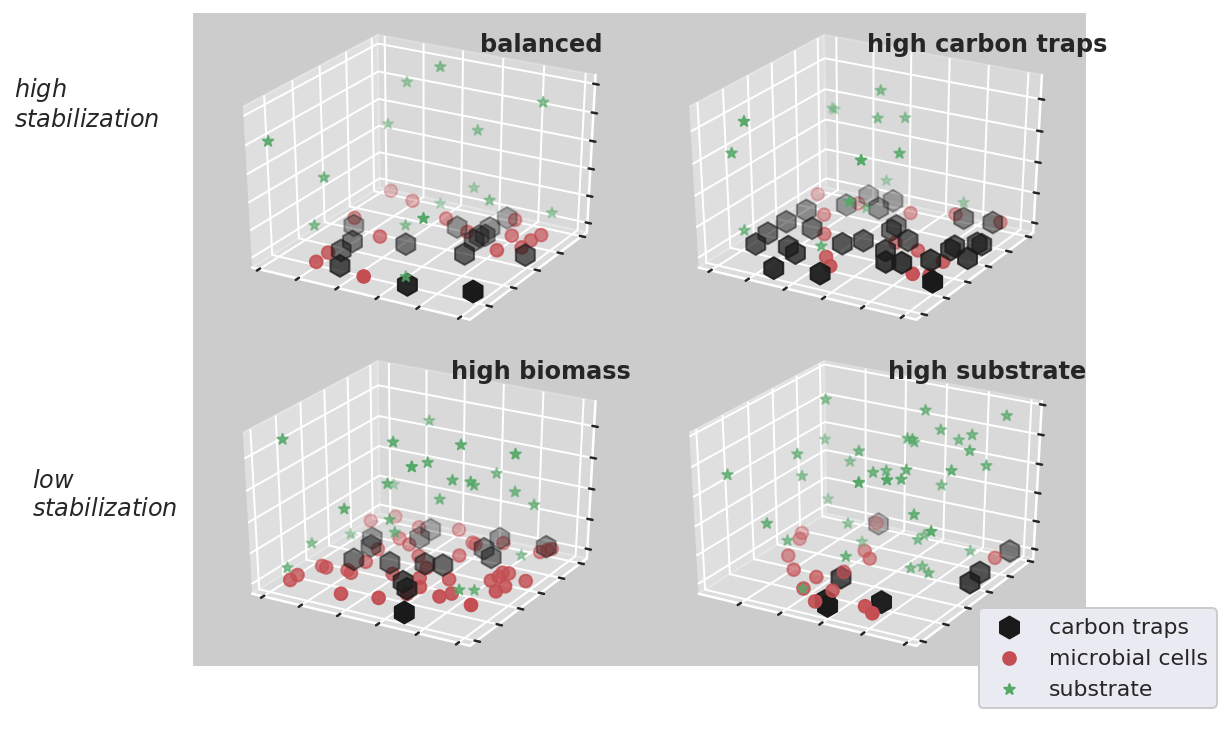
\includegraphics[scale=0.8]{thesis_figures/test/model_scenarios.png}
	 	\caption{examples of the different model scenarios with their corresponding outcome on the far left side of the figure}
	 	\label{fig:stabilization_model_scenarios}
	 \end{figure}

	 In the current experiment, a series of three consecutive, high rate applications of highly labile organic substrate was setup, each portion causing a rapid increase in microbial biomass followed by period of diminishing MB. In the first week for example, this strong microbial turnover likely yielded a large quantity of available carbonaceous organic substances in the form of necromass and other microbial products in the days following peak microbial growth
	 (‘secondary pulse’),
	 % microbial death
 	 and It is reasonable to assume that a substantial portion of this secondary pulse was still present in some sort of readily available form 7 days after MRE application (‘leftover carbon’), when a subsequent input was applied.
% 	 \myRed{Substantial increases in net HWES during week 1 and 2 seem to correspond with such 'leftover carbon'}.
 	 Evidently, in all three LTTs, also the live microbial biomass as well as  aggregate structure had changed considerably between one MRE application and the next, particularly in the first and second weeks of incubation.\\
	 Examined in light of the proposed stabilization model, these changes imply a modified setting into which MRE is applied in the 2nd and 3rd week. The large amount of labile carbon applied at $ T_0 $ had caused a surge of microbial growth (model variable (1)) which as suggested above, consequently resulted in a secondary pulse of large quantities of readily available microbial products (model variable (2)) yet proposedly, these pulses were not accompanied by proportional increases in potential sites of OM stabilization(variable (3)). Considering the soil system right after the 2nd MRE application it is suggested that the sum of leftover carbon from the first application, along with newly introduced MRE carbon, resulted in a situation corresponding to scenario (1) in the stabilization model,  in which a high substrate-to-biomass ratio but especially high proportion of substrate to available stabilization sites would result in lower \gls{cue}.
	 Direct meaningful  assessment of \gls{om} stabilization was not possible using data from the current experiment,
	 it is assumed therefore that my \gls{cue} results provide a viable indication of the efficiency of short term \gls{om} stabilization (i.e the fraction of substrate-C remaining in the soil).\\
%			 microbial products and necromass as primary source of stable \gls{som}
	 microbial growth and respiration data in the 1st incubation week, seems to be in full agreement with the above proposed mechanism for reduced \gls{cue}. All three LTTs had seen a considerable increase in the weekly cumulative respiration while simultaneously presenting a notable decrease in the weekly microbial growth. The proportion of weekly respired $ CO_2 $-$ C $ to the weekly MRE-C applied had increased by roughly 10\% between the 1st and 2nd week while this same proportion for weekly microbial growth, decreased by more than tenfold for ORG and UNC and by a little more than half for MIN. Given the validty of assumptions \ref{item: complete_uptake} and \ref{item: negligible_priming} of complete uptake and neglible priming, the inefficient use of MRE input in the 2nd, compared with the 1st week becomes evident. \\
%	 \myRed{how exactly is the efficiency of microbial growth related to the efficiency of carbon stabilization, i.e \%stabilization?}\\
	 according to the suggested 'stabilization model', higher substrate-to-biomass and a higher proportion of these two features to the availability of stabilization sites (or 'carbon traps'), would results in a smaller fraction of substrate-C remaining in the soil matrix, not necessarily less MBC being accumulated (as was observed in my results). However, it is suggested here that, besides ensuring carbon stabilization efficiency, a balanced proportion of available substrate, microbial biomass and soil pore availability for carbon protection, will also be reflected in more efficient accumulation of MB which would presumably result in a higher \%stabilization.\\
%todo why higher biomass accumulation results in higher stabilization
 	 another soil feature that presented a strong reaction to consecutive MRE additions was the WEOC fraction. Large pulses of WEOC were observed after each MRE addition (for the first week, mainly in UNC) and these pulses increased considerably with consecutive additions (particularly for UNC and MIN). Likewise the extent of these pulses was positively correlated with lower respiration rate and lower biomass among the three LTTs. This clearly points out to a phenomena mentioned earlier, whereby reduced microbial activity is reflected in greater accumulation of labile organic carbon, at least in the short term of a couple of days. In the 2nd week these trends in WEOC coincide with greatly reduced \gls{cue} in all three LTTs, and especialy in UNC, which incidently also had the highest WEOC accumaltion 24 h after MRE addition on that week. It seems that, mainly for UNC and MIN, the surge of easily available organic substrate ( from both 'leftover carbon' as well as from newly introduced MRE) has caused the microbial biomass to be overwhelmed, considerably reducing the uptake and utilization rate of available substrate in the first day or two after MRE addition and concurently also resulting in reduced weekly \gls{cue}.
	 This was not the case for ORG, as the clear reduction in \gls{cue} was not accompanied by substantial pulses of WEOC.

\section{Short term dynamics of \gls{som} pools in amended soils}
%todo rephrase above title
%todo rewrite opening section. shorter recap of the previuos section and include the opening of next subsection

In this work, I’ve attributed particular importance to the proportion of Microbial growth to microbial respiration, expressed as the \gls{cue} index, as it was postulated to reflect to a large degree, the efficiency of incoming \gls{om} stabilization and incorporation into \gls{som}. This approach has proven to be at least partially successful in illustrating the effect of sequential labile substrate applications, as it indicated a reduction in \gls{cue} with each subsequent MRE addition. A much more limited success was achieved in trying to distinguish the effect of management history on the short term dynamics of \gls{som} pools, using  the \gls{cue} index. As noted earlier, ORG and MIN displayed a very similar  reduction in \gls{cue} throughout the incubation, while a somewhat erratic pattern was observed for UNC. Additionally, large uncertainties are associated with the weekly \gls{cue} results making it hard to assert  meaningful distinction between LTTs.\\ 

	\subsection{Variability in WEOC removal}
	The dynamics of MBC by itself, also did not seem to reveal any significant differences between LTTs in their response to MRE input.
	However, the dynamics of CO2-Resp and moreover those of WEOC, in MRE amended samples, suggest a notable effect of management history on \gls{som} dynamics in this short term incubation. WEOC levels had peaked at almost 1000 mg/kg  24 h after the first MRE addition in UNC samples and the corresponding peak 24 h after the third MRE application in these UNC samples was almost double the size of the first peak. Data is missing for the second peak in UNC samples, yet it is assumed to have followed the trend suggested by the large differences between the first and third WEOC peak. This trend is similarly observed in MIN samples, albeit with a significantly lower intensity. Remarkably, these sharp increases in WEOC 24 h after MRE addition, were not observed in ORG on any sampling event.\\
	The intensity of WEOC pulses after each MRE addition increased both in time ( with consecutive MRE applications) and also between LTTs, in the following order, UNC $ > $ MIN $ > $ ORG. This order of response intensity between the three LTTs, most clearly notable 1 day after MRE additions, seems to be largely opposite to the order of baseline SOC content and baseline MBC between these LTTs, which were as follows, ORG $ > $ MIN $ > $ UNC (differences in MBC between ORG and MIN and between MIN and UNC in SOC, are not significant). This suggest  that higher initial \gls{som} content and/or higher extant microbial biomass may have been related to moderated fluctuations in WEOC following MRE additions and to moderated increases in the intensity of these fluctuations as the incubation preceded. \\
	Results from the preliminary incubation are indicative of the important role of microbial respiration in the removal of WEOC from the soil. Both Str or KWC amended soils as well as non-amended samples from the preliminary incubation presented an inverse trend between WEOC and Resp dynamics. However, no significant difference between ORG and MIN (in Str or KWC amended soils) was observed in terms of the efficiency of WEOC removal. In the MRE incubation, a comparison of WEOC dynamics with those of Resp revealed an opposite trend in the order of LTTs throughout most of the incubation. In this way soil samples in which Resp was high presented low WEOC pulses and vice versa. Although the sample size of different LTTs was quite low (N=3), the relation between microbial activity (Resp) and WEOC removal seems apparent. \\
%	additionally, cumulative respiration in the three LTTs suggests the connection between elevated microbial activity (i.e respiration) and the quick removal of labile organic carbon.

	In the current experiment, an exceptionally high load of labile organics was applied with each MRE addition, roughly an order of magnitude higher than baseline MBC values.  Although labile DOM is usually rapidly consumed by the soil microbial population it is possible that in situations were a proportionally large amount of labile substrate is rapidly introduced, the microbial population would be unable to process it completely, in the very short term of several hours to a day or two. Thus, considerable amounts of substrate could be accumulated as WEOM. This seems to have been the case in the current experiment, where in the first week of incubation both ORG and MIN, presumably possessing a significantly higher reserve of active and potentially active microbial biomass, presented a very low increase in WEOC 24 h after MRE addition . This is suggestive of the metabolic capacity of these soil microbial populations allowing them to rapidly consume and break down the input substrate to the extent that it is unrecoverable as WEOM, either by mineralization of the substrate into CO2, its immobilization as MB or its transformation into metabolic products that would have been bound to the solid soil phase.
	%, rendering it unextractable with water.
	 In the subsequent MRE additions, it is assumed that-although MRE input load was unchanged-the conditions with regard to microbial biomass and overall labile \gls{om} availability had been altered significantly, resulting in the increased intensity of WEOC pulses in these subsequent MRE additions (in MIN and UNC). As discussed in a previous section, it is suggested that by the end of the first week of incubation, the levels of labile \gls{om} availability had increased substantially (\textit{leftover carbon}). While MBC also increased  considerably in all three LTTs during the first week, it is proposed that the substrate-to-biomass  ratio had increased considerably between the first and second MRE additions in MIN and UNC, which may have been the primary reason for the observed pulses of WEOC following MRE addition, as the microbial populations in these soil samples were ineffective in removing the large influx of DOM during the first 24 h.

	In line with the proposed \textit{stabilization model} as well as the evidence presented earlier regarding the nature of DOM, I propose three  major drivers which controlled the dynamics of WEOC in the days following each MRE addition, each one represented by a measured soil feature:
	\begin{enumerate}
		\item microbial assimilation (MBC)
		\item microbial mineralization (CO2-Resp)
		\item potential for \gls{om} stabilization (AS, expressing the potential availability of the soil mineral phase for interaction with incoming decomposition products).
	\end{enumerate}


	while  CO2 mineralization can explain some of the variation in WEOC between LTTs, it is clearly not enough to explain all of the variation, as evident when comparing cumulative Resp trends with those of WEOC. The largest difference by far between LTT's in the percent change of cumulative respiration, is observed during the first pulse while subsequent pulses presented a much smaller and relatively minor difference between LTTs in terms of percent change in cumulative respiration.
	Microbial assimilation might have accounted for some of the variation yet no significant differences between LTT's were observed during the incubation.
	It seems therefore, that neither microbial growth (anabolism) nor microbial respiration (catabolism) can fully account for the variation between LTTs. The third driver listed above, namely soil potential for \gls{om} stabilization, remains thus as a possible candidate to account for the primary share of this observed variability. It is noted here that my analysis of soil aggregate stability provides only inferential information regarding the dynamics of soil stabilization potential, both due the low sampling frequency during the incubation as well as the nature of the test itself which provides a general indication of the aggregation status of the soil rather than a more detailed characterization of soil spatial organization. For example, an elaborate description of soil pore architecture including for example, pore size distribution and connectivity, could have been much more effective in examining the relation between stabilization potential and microbial efficiency in general and the short term removal of labile \gls{om} from soil solution in particular. \\
	Despite these limitations, AS is nonetheless presumed to provide valuable indications of a soil stabilization potential. The significantly lower \%WSA in UNC compared with the two other LTTs, throughout the incubation, is in accordance with the higher intensity of WEOC pulses in that LTT, suggesting structural features may have been a significant factor in this regard. However, differences between ORG and MIN did not correspond with the variations between these LTTs in terms of WEOC dynamics.  \\

%\section{conclusions \hiddenTxt{limitations of the experimental setup}and suggestions for further research}
%
%		This research examined the effect of long term soil management and particularly fertilization management, on \gls{som} pools and related soil features such as AS. Our analysis of the dynamics as well baseline values of non-amended samples, provided strong evidence for the effect of 5 years of contrasting fertilization schemes on \gls{som} pools. These results indicated a clear distinction between organically and mineraly fertilized soil in both total SOC as well as biological \gls{som} pools. That this distinction was observed in soil samples obtained after a substantial resting period (\textit{no input + fallow}) in the original long-term experiment (GOP) is of particular interest.      , results from our MRE as well as Str and KWC amended samples were far more ambiguous.

	%The dynamics of WEOC in MRE amended samples present a definite distinction between LTTs, and this distinction matches clearly, though inversely, the variation between LTTs in baseline MBC and Resp. This \myRed{seemingly} negative correlation between WEOC on the one hand and extant microbial biomass on the other hand, similarly observed in all of the incubations during this research, provides strong evidence of the close association of microbial activity and WEOC. It is highly likely then, that increased microbial biomass and particularly active microbial biomass (as reflected in Resp) in the cultivated LTTs as opposed to UNC, had an essential role in driving this differential response between LTTS. This was corroborated to \gls{som}e extent by Resp dynamics during the MRE incubation itself, though not so much by MBC. The fact that microbial respiration is more strongly indicative of the active share of microbial biomass has been discussed earlier in this work. It is therefore not unlikely that the differential response of microbial biomass in terms of removal of WEOC for example, was not significantly reflected in MBC data.

%preliminary incubation
%	all treatment combinations presented a significant increase in WEOC on the first sampling event which was shortly after followed by a steep decline. the initial increase in WEOC was likely the result of substrate solubilization by water addition and/or microbial action, producing substantial amounts of WEOC. this easily available carbon pool was rapidly and continuously removed in the following days by microbial consumption, resulting in decreased WEOC. this decrease closely coincides with the time frame of maximum respiration, between 0-48 h, after which respiration rates had mostly leveled off. concurrence of WEOC removal with increased Resp levels, also observed for control samples in the preliminary experiment, effectively illustrates the  notion of WEOC as an immediate and labile source of energy for micro-organisms.


The dynamics of HWES had also presented considerable variation between LTTs during the 28 days MRE incubation. The hot water extractable fraction of \gls{som} is often associated with aggregation processes, particularly its carbohydrate portion.  However HWEC and specifically HWES are also regarded as a labile source of energy utilized by the microbial population. In the current work, HWES dynamics during the MRE incubation mostly seemed to accord with the later view. When examining the net HWES accumulation in the course of the incubation, there appears to be a similar relation between HWES accumulation and the metabolic capacity of the soil (represented by MBC and moreover microbial Resp), as described above for WEOC. Although this relation is evidently not as clear as for WEOC, it does become more evident at day 21 and certainly at day 28 wherein the order of HWES content between LTTs is opposite with the general order of MBC and Resp as observed throughout my experiments. Clearly the significantly higher net HWES in UNC at days 14, 21 and 28, compared with both cultivated LTTs, is indicative of the lower metabolic capacity of this soil, as was also observed for WEOC. Here again, it remains unclear whether and in what way, the variation in HWES consumption and removal from DOM fraction is connected with microbial \gls{cue} and the carbon stabilization potential. However it appears that microbial capacity for labile carbon removal from DOM fraction is at least to some extent positively related with \gls{cue}, as evident from the inverse general trend in \gls{cue} as opposed to WEOC and HWES across the incubation period.
